\section{Uitbeidingen op TikZ}

\begin{frame}
  \frametitle{Libraries}

  Zie \S IV in versie 2.10, of \S V in versie 3.0 voor de \emph{libraries} (= intern).

  \pause
  Te gebruiken via:
  
  \mintinline{latex}|\usetikzlibrary{lindenmayersystems}|

  \begin{alertblock}{Vraag}
    Wat doet deze library?
  \end{alertblock}
\end{frame}

\begin{frame}
  \frametitle{Lindenmayersystemen}

  \begin{columns}
    \begin{column}{.6\textwidth}
      \inputminted[fontsize = \scriptsize]{latex}{tikz/l-system.tikz}
    \end{column}
    \begin{column}{.4\textwidth}
      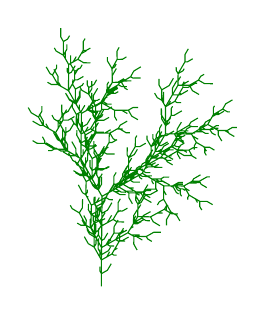
\begin{tikzpicture}
\draw[green!50!black, rotate=90]
  [l-system={rule set={F -> FF-[-F+F]+[+F-F]},
    axiom=F, order=4, step=2pt,
    randomize step percent=25, angle=30,
    randomize angle percent=5}]
  lindenmayer system;
\end{tikzpicture}

    \end{column}
  \end{columns}
\end{frame}

\begin{frame}
  \frametitle{Packages}

  Zie \url{http://ctan.org/search?phrase=tikz} voor \emph{packages} (= extern): 90+ resultaten

  \mintinline{latex}|\usepackage{...}|

  \pause
  \begin{enumerate}
    \item \texttt{tikz-qtree}
    \item \texttt{tqft}
    \item \texttt{tikz-cd}
    \item \ldots
  \end{enumerate}
\end{frame}

\begin{frame}
  \frametitle{\texttt{tikz-qtree}}
  
  Automatisch bomen tekenen:
  \begin{columns}
    \begin{column}{.6\textwidth}
      \inputminted[fontsize = \scriptsize]{latex}{tikz/tikz-qtree.tikz}
    \end{column}
    \begin{column}{.4\textwidth}
      \begin{tikzpicture}[scale = .8]
  \Tree [.S [.NP [.Det the ] [.N cat ] ]
            [.VP [.V sat ]
                 [.PP [.P on ]
                      [.NP [.Det the ]
                      [.N mat ] ] ] ] ]
\end{tikzpicture}

    \end{column}
  \end{columns}
\end{frame}

\begin{frame}
  \frametitle{\texttt{tqft}}
  
  Om diagrammen in topologische quantumveldentheorie te tekenen:
  \begin{columns}
    \begin{column}{.6\textwidth}
      \inputminted[fontsize = \scriptsize]{latex}{tikz/tqft.tikz}
    \end{column}
    \begin{column}{.4\textwidth}
      \begin{tikzpicture}[scale = .8]
  \node[draw, tqft/pair of pants]
    (a) {};
  \node[draw, tqft/cylinder to next,
        anchor = incoming boundary 1]
    (c) at (a.outgoing boundary 1) {};
  \node[draw, tqft/reverse pair of pants,
        anchor = incoming boundary 1]
    at (a.outgoing boundary 2) (b) {};
\end{tikzpicture}

    \end{column}
  \end{columns}
\end{frame}

\begin{frame}
  \frametitle{\texttt{rubikcube}}

  Om Rubik's cubes te tekenen:
  \begin{columns}
    \begin{column}{.6\textwidth}
      \inputminted[fontsize = \scriptsize]{latex}{tikz/rubikcube.tikz}
    \end{column}
    \begin{column}{.4\textwidth}
      
\begin{tikzpicture}[scale=.4]
  \DrawRubikLayerFace{G}{Y}{R}
                     {Y}{Y}{Y}
                     {B}{Y}{Y}
  \DrawRubikLayerSideT {Y}{B}{B}
  \DrawRubikLayerSideLR{R}   {Y}
                       {R}   {O}
                       {Y}   {O}
  \DrawRubikLayerSideB {O}{G}{G}
  \draw[->,ultra thick,color=green]
    (0.5,5) -- (0.5, 4);
\end{tikzpicture}

\begin{tikzpicture}[scale=.4]
  \RubikCubeSolved
  \DrawRubikCubeFlat
\end{tikzpicture}

    \end{column}
  \end{columns}
\end{frame}

\subsection{Commutatieve diagrammen}

\begin{frame}[fragile]
  \frametitle{Commutatieve diagrammen}

  \small
  We gebruiken \mintinline{latex}|\usepackage{tikz-cd}|.
  \begin{columns}
    \begin{column}{.67\textwidth}
      \inputminted[fontsize = \scriptsize]{latex}{tikz/diagrams/1.tikz}
    \end{column}
    \begin{column}{.33\textwidth}
      \begin{equation}
  \begin{tikzcd}
    A \arrow{rd} \arrow{r}{\phi} & B \\
                                 & C
  \end{tikzcd}
\end{equation}

    \end{column}
  \end{columns}
  \small
  \begin{enumerate}
    \item\pause de \emph{eerste parameter} van \mintinline{latex}|\arrow| is altijd de richting: een combinatie van \texttt{u}, \texttt{d}, \texttt{r}, \texttt{l}, de \emph{tweede} een (optioneel) label
    \item\pause vertices zoals we tabellen schrijven 
  \end{enumerate}
  \begin{alertblock}{Opgepast}
    \dbend\quad Pijlen kunnen enkel naar bestaande vertices.
  \end{alertblock}
\end{frame}

\begin{frame}
  \frametitle{Oefening}

  \footnotesize
  \begin{equation*}
  \begin{tikzcd}
    A  \arrow{r}{f} \arrow{d}{l} & B \arrow{r}{g} \arrow{d}{m} & C \arrow{r}{h} \arrow{d}{n} & D \arrow{r}{j} \arrow{d}{p} & E \arrow{d}{q} \\
    A' \arrow[swap]{r}{r}        & B' \arrow[swap]{r}{s}       & C' \arrow[swap]{r}{t}       & D' \arrow[swap]{r}{u}       & E' \\
  \end{tikzcd}
\end{equation*}

  \begin{equation*}
  \begin{tikzcd}
    T
    \arrow{drr}{x}
    \arrow[swap]{ddr}{y}
    \arrow[dotted]{dr}[description]{\exists} & & \\
      & X \times_Z Y \arrow[swap]{r}{p} \arrow{d}{q}
        & X \arrow{d}{f} \\
      & Y \arrow[swap]{r}{g} &Z
  \end{tikzcd}
\end{equation*}

\end{frame}
